\chapter{Hardware and Software Requirements Specification}
\section{Hardware Specification}
\subsection{Raspberry Pi 4}
\paragraph{} Raspberry Pi microprocessor is most preferred when developing advanced \\applications. Raspberry Pi is an open source platform where one can get a lot of related information so you can customize the system depending on the need. 
\subsubsection*{Features of Raspberry Pi 4}
\begin{enumerate}
\item Broadcom BCM2711, Quad core Cortex-A72 (ARM v8) 64-bit SoC @ 1.5GHz
\item 2GB, 4GB or 8GB LPDDR4-3200 SDRAM (depending on model)
\item 2.4 GHz and 5.0 GHz IEEE 802.11ac wireless, Bluetooth 5.0, BLE
\item Gigabit Ethernet
\item 2 USB 3.0 ports; 2 USB 2.0 ports.
\item Raspberry Pi standard 40 pin GPIO header (fully backwards compatible with previous boards)
\item 2 × micro-HDMI ports (up to 4kp60 supported)
\item 2-lane MIPI DSI display port
\item 2-lane MIPI CSI camera port
\item 4-pole stereo audio and composite video port
\item H.265 (4kp60 decode), H264 (1080p60 decode, 1080p30 encode)
\item OpenGL ES 3.0 graphics
\item Micro-SD card slot for loading operating system and data storage
\item 5V DC via USB-C connector (minimum 3A*)
\item 5V DC via GPIO header (minimum 3A*)
\item Power over Ethernet (PoE) enabled (requires separate PoE HAT)
\item Operating temperature: \ang{0}C – \ang{50}C ambient
\end{enumerate}
* A good quality 2.5A power supply can be used if downstream USB peripherals consume less than 500mA in total.\\
\begin{figure}[h]
\centering
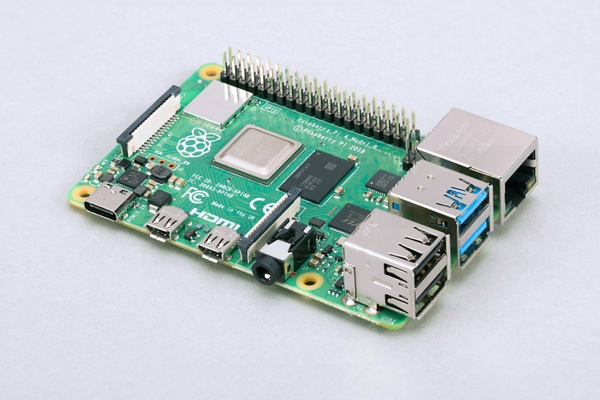
\includegraphics[scale=0.5]{rpi.jpg}
\caption{Raspberry Pi 4} \vspace{1cm}
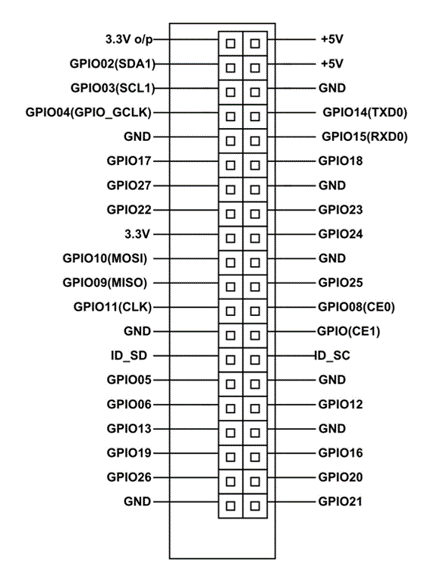
\includegraphics[scale=0.5]{rpipin.png}
\caption{Raspberry Pi Pin-out}
\end{figure}
\subsection{Raspberry Pi Camera}
The Raspberry Pi Camera Modules are official products from the Raspberry Pi \\Foundation. The original 5-megapixel model was released in 2013, and an 8-megapixel Camera Module v2 was released in 2016. For both iterations, there are visible light and infrared versions. A 12-megapixel High Quality Camera was released in 2020.
\begin{figure}[h]
\centering
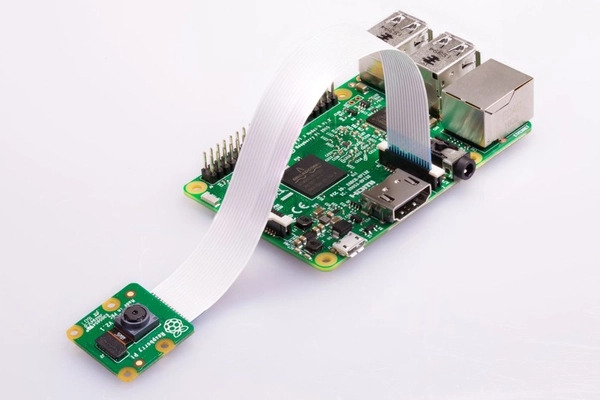
\includegraphics[scale=0.32]{rpicam.jpg}
\caption{Raspberry Pi Camera v2.1}
\end{figure}
\subsection{BO DC Motor}
BO (Battery Operated) light weight DC geared motor which gives good torque and rpm at lower voltages. This motor can run at approximately 200 rpm when driven by a single Li-Ion cell. Great for battery operated light weight robots. It can do reverse and forward directions.
\subsubsection*{BO Motor Specifications:}
\begin{enumerate}
\item Working Voltage 3-12V
\item No Load Speed: 200 rpm /- 10rpm
\item No Load Current: 125mA (max.170mA)
\item Torque: 500gf.cm min 40gm weight
\end{enumerate}
\begin{figure}[h!]
\centering
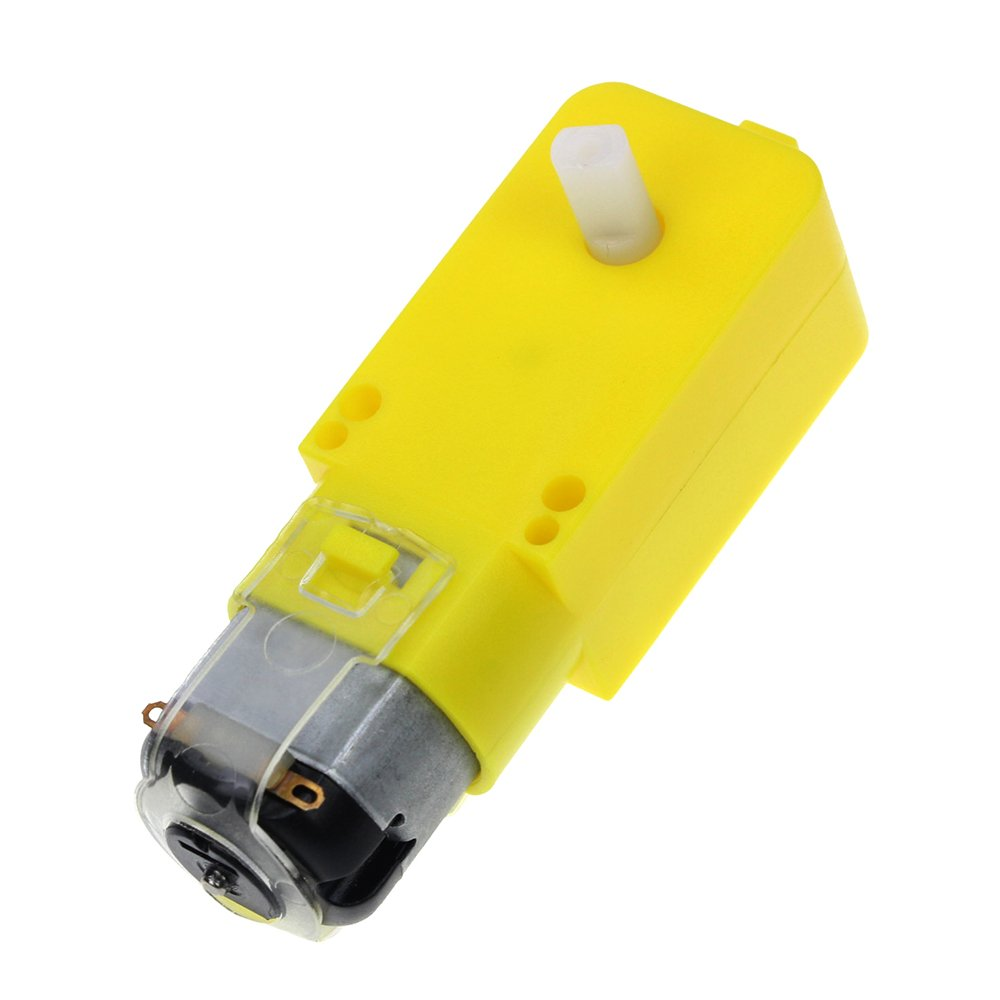
\includegraphics[scale=0.11]{bomotor.jpg}
\caption{BO DC Motor}
\end{figure}
\subsection{L298N Motor Driver}
L298N Motor Driver Module is a high power motor driver module for driving DC and Stepper Motors. This module consists of an L298 motor driver IC and a 78M05 5V regulator. L298N Module can control up to 4 DC motors, or 2 DC motors with directional and speed control.
\subsubsection*{L298N Module Features \& Specifications:}
\begin{enumerate}
\item Driver Model: L298N 2A 
\item Driver Chip: Double H Bridge L298N 
\item Motor Supply Voltage (Maximum): 46V 
\item Motor Supply Current (Maximum): 2A 
\item Logic Voltage: 5V 
\item Driver Voltage: 5-35V 
\item Driver Current:2A 
\item Logical Current:0-36mA 
\item Maximum Power (W): 25W 
\item Heatsink for better performance 
\end{enumerate}
\begin{figure}[h]
\centering
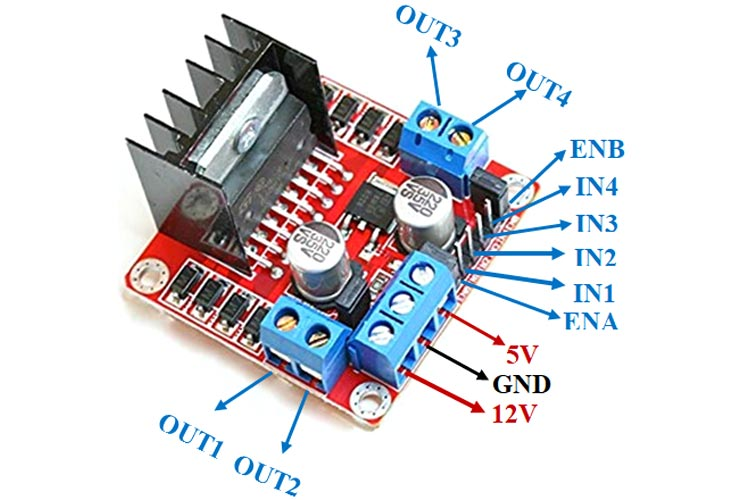
\includegraphics[scale=0.4]{L298N.jpg}
\caption{L298N Motor Driver}
\end{figure}
\subsection{LiPo Battery}
A lithium polymer battery, or more correctly lithium-ion polymer battery, is a rechargeable battery of lithium-ion technology using a polymer electrolyte instead of a liquid electrolyte. High conductivity semisolid (gel) polymers form this \\electrolyte. These batteries provide higher specific energy than other lithium battery types and are used in applications where weight is a critical feature, such as mobile devices, radio-controlled aircraft and some electric vehicles 
\begin{figure}[h]
\centering
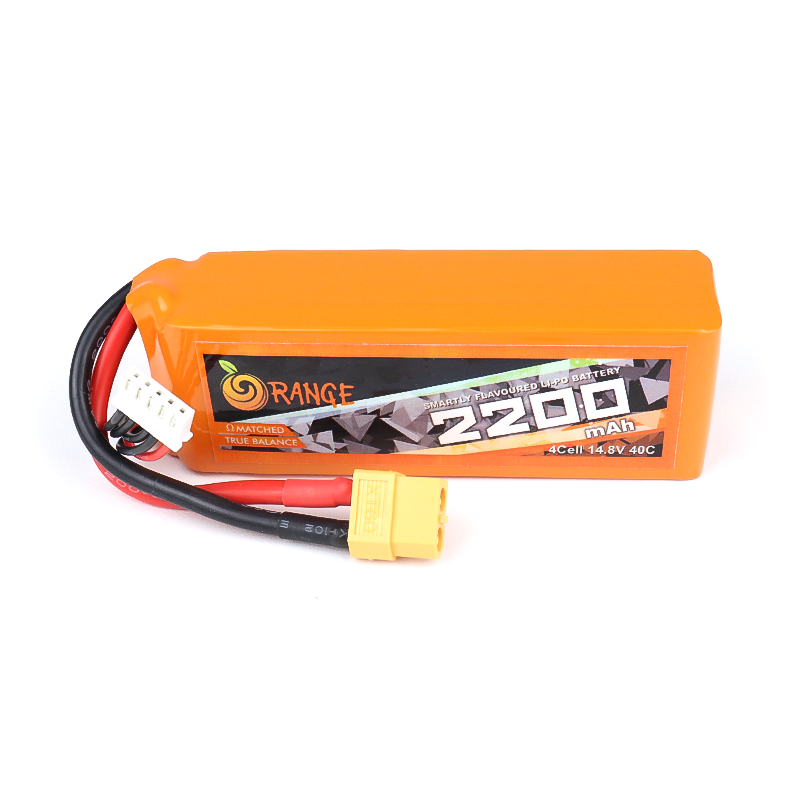
\includegraphics[scale=0.25]{lipo.png}
\caption{LiPo Battery}
\end{figure}
\subsection{Router(Gateway)}
\begin{enumerate}[ ]
\item The router is a physical or virtual inter-networking device that is designed to receive, analyze, and forward data packets between computer networks. A router examines a destination IP address of a given data packet, and it uses the headers and forwarding tables to decide the best way to transfer the packets. 
Some important points of routers are given below: 
\item A router is used in LAN (Local Area Network) and WAN (Wide Area Network) environments. For example, it is used in offices for connectivity, and you can also establish the connection between distant networks. 
\item It shares information with other routers in networking. 
\item It uses the routing protocol to transfer the data across a network. 
\end{enumerate}
\begin{figure}[h]
\centering
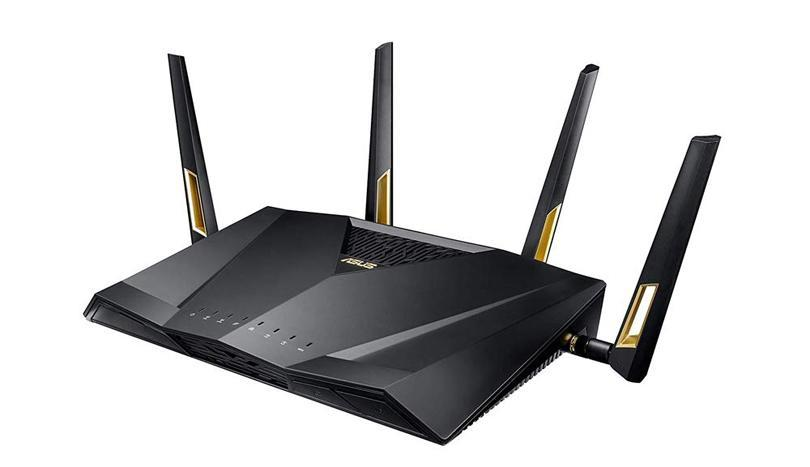
\includegraphics[scale=0.3]{router.jpg}
\caption{Router}
\end{figure}
\section{Software Requirements}
\subsection{Raspbian}
\begin{enumerate}[ ]
\item Raspberry Pi OS (formerly Raspbian) is a Debian-based operating system for Raspberry Pi. Since 2015 it has been officially provided by the Raspberry Pi Foundation as the primary operating system for the Raspberry Pi family of compact single-board computers. 
\item Previous Pi OS versions have been 32bit and based on Raspbian core, taking the name Raspbian. Since recent 64bit versions no longer use the Raspbian core, the name has been changed to Raspberry Pi OS for both 64bit and 32bit versions.
\item Raspberry Pi OS is highly optimized for the Raspberry Pi line of compact single-board computers with ARM CPUs. Raspberry Pi OS uses a modified LXDE as its desktop environment with the Openbox stacking window \\manager. 
\end{enumerate}
\begin{figure}[h]
\centering

\includegraphics[scale=0.3]{raspbian.png}
\caption{Rasbian}
\end{figure}
\newpage
\subsection{Python}
\begin{enumerate}[ ]
\item Python is an interpreted, high-level and general-purpose programming \\language. Python's design philosophy emphasizes code readability with its \\notable use of significant whitespace. Its language constructs and object-oriented approach aim to help programmers write clear, logical code for small and \\large-scale projects.
\item Python is dynamically typed and garbage-collected. It supports multiple \\programming paradigms, including structured (particularly, procedural), \\object-oriented and functional programming. Python is often described as a "batteries included" language due to its comprehensive standard library.
\end{enumerate}
\begin{figure}[h]
\centering

\includegraphics[scale=0.3]{python.png}
\caption{Python}
\end{figure}

\subsection{Flask}
\begin{enumerate}[ ]
\item Flask is a micro web framework written in Python. It is classified as a \\microframework because it does not require particular tools or libraries. It has no database abstraction layer, form validation, or any other components where \\pre-existing third-party libraries provide common functions.
\item However, Flask supports extensions that can add application features as if they were implemented in Flask itself. Extensions exist for object-relational mappers, form validation, upload handling, various open authentication technologies and several common framework related tools.
\end{enumerate}
\begin{figure}[h]
\centering
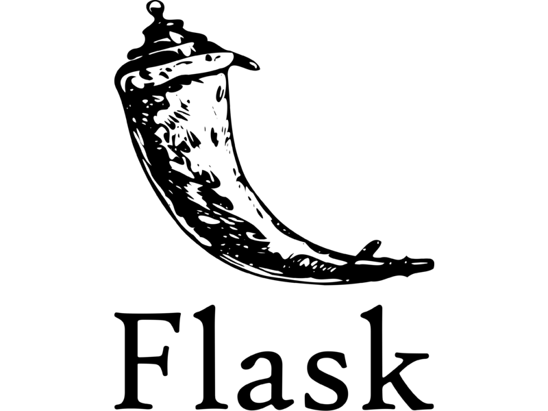
\includegraphics[scale=0.3]{flask.png}
\caption{Flask}
\end{figure}